% 公立はこだて未来大学 卒業論文 テンプレート ver1.50
% (c) Junichi Akita (akita@fun.ac.jp), 2003.10.31
% update by N.T.,  2004.11.10
%
\documentclass{funthesis}
%¥documentclass[english]{funthesis} % use [english] option for English style

\usepackage[dvips]{graphicx} % 図(EPS形式)を本文中で読み込む場合はこれを宣言
\usepackage{url}

% この部分に,タイトル・氏名などを書く.
% タイトルなどの定義の始まり
\jtitle{知識ベース型推薦を用いた\\フードツーリズム支援システムの構築}% 論文の和文タイトル
%
\etitle{Development of a Food Tourism Support System Using Knowledge-based Recommendation}% 論文の英文タイトル
%
\htitle{Development of a Food Tourism Support System Using Knowledge-based Recommendation}   % ヘッダー用の論文の短縮英文タイトル
%     必ず1行に収まるように英文タイトルを短縮する.
%
\jauthor{三好 良弥}     % 氏名(日本語)
\eauthor{Ryoya Miyoshi}   % 氏名(英語)
\jaffiliciation{情報アーキテクチャ学科} % 所属学科名(日本語)
\eaffiliciation{Department of Media Architecture} % 所属学科名(英語)
\studentnumber{1014127}   % 学籍番号
\jadvisor{奥野 拓}    % 正指導教員名(日本語)
%¥jcoadvisor{} % 副指導教員(日本語)がいる場合は
                        % コメントアウトし名前を書く
                        % 副指導教員がいない場合は,ここは削除しても可
\eadvisor{Taku Okuno}  % 正指導教員名(英語)
%¥ecoadvisor{}   % 副指導教員(英語)がいる場合は
                         % コメントアウトし名前を書く
                         % 副指導教員がいない場合は,ここは削除しても可
\jdate{平成30年01月29日}    % 論文提出日   (日本語)
\edate{January 29, 2018}     % 論文提出年月 (英語)
% タイトルなどの定義の終わり

\begin{document}

%--------------------------------------------------------------------
\maketitle       % タイトルページを作成

%--------------------------------------------------------------------
% 英文概要(250語程度)
\begin{eabstract}
In recent years, food tourism that a tourism aimed at eating local food is popular.
However, the criteria for regional dishes differ depending on the taste of tourists, it is difficult to find a local food at conventional gourmet websites.
In order to solve this problem, this research proposes a local food recommendation system considering the taste of tourists.
I extract information on restaurants and dishes using Web scraping at gourmet websites.
I build a database using the extracted information and recommend a local food to the taste of tourists.
As a recommendation method, by using Knowledge-based Recommendation  that is effective when there is a specific condition that the user requires for the product.
\end{eabstract}

% 英文キーワード(5個程度をコンマ(,)で区切って羅列する)
\begin{ekeyword}
Food Tourism, Knowledge-based Recommendation, Preference Information
\end{ekeyword}

%--------------------------------------------------------------------
% 和文概要(300字程度)
\begin{jabstract}
近年,地域らしい料理を食べることを目的とした旅であるフードツーリズムが盛んである.
しかし,観光客の嗜好によって地域らしい料理の判断基準が異なるため,従来のグルメサイトでは地域らしい料理を探すことが困難である.
この問題を解決するために,観光客の嗜好を考慮した地域らしい料理推薦システムを提案する.
推薦手法として,「評価が高い商品」や「1000円以下の商品」などユーザが商品に求める具体的な条件がある場合に有効な知識ベース型推薦を用いることで,嗜好にあった料理の推薦を可能にする.
提案手法として,スクレイピングを用いてグルメサイトから飲食店及び料理の情報を抽出する.
その後,抽出した情報を用いてデータベースを構築し,観光客の嗜好にあった地域らしい料理の推薦を行う.
本研究の提案手法の有用性を確認するため,提案システムとグルメサイトの比較実験を行った.
実験の結果,ほげほげとわかった.
\end{jabstract}

% 和文キーワード(5個程度をコンマ(,)で区切って羅列する)
\begin{jkeyword}
フードツーリズム,知識ベース型推薦,嗜好情報
\end{jkeyword}

%--------------------------------------------------------------------
\tableofcontents % 目次を作成



%--------------------------------------------------------------------
% ¥includegraphics[width=??cm]{hoge.eps} % 図(EPS形式)を読み込む場合


%--------------------------------------------------------------------

\chapter{序論} 

\section{フードツーリズムとは}
近年,これまで観光資源としては気付かれていなかった地域固有の資源を新たに活用し,体験・交流型の要素を取り入れた旅行の形態である,ニューツーリズムの振興が図られている\cite{1}.
ニューツーリズムが盛んになってきたことにより,従来では観光資源にならなかったものが,新たな観光資源として活用されるようになってきた.

じゃらんが実施したアンケートの「宿泊旅行調査」の調査結果を図1.1に示す\cite{2}.
この調査によると,観光客が観光地を選んだ理由のひとつとして「地域らしい料理・特産品に興味があったから」と回答した人が年々増加傾向であり,2016年度は41.6\%であった.
このことから,観光客は地域らしい料理をという観光資源を旅行の際に重要視していることがわかる.

\begin{figure}[!b]
  \begin{center}
    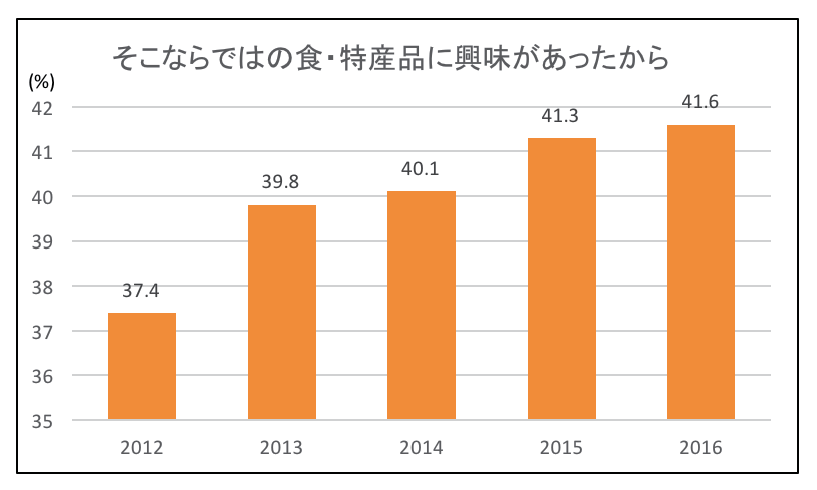
\includegraphics[clip,width=13cm]{jaran.eps}
    \caption{観光地を選ぶ理由}
  \end{center}
\end{figure}

地域らしい料理を観光資源としたニューツーリズムのことをフードツーリズムと呼ぶ.
日本フードツーリズム協会によると,フードツーリズムは地域らしい料理・食文化,それを引き立てる体験,場所,人の4つの要素から成り立っているとしている\cite{3}.

\section{フードツーリズムの問題点}
フードツーリズムの重要な要素である地域らしい料理を観光客が探す方法の1つとしてグルメサイトを用いて調べるという方法がある.
しかし,観光客によって地域らしい料理に求める条件が異なり,「食べログ」\cite{4},「ぐるなび」\cite{5}などのグルメサイトでは,観光客が求める条件を入力したりすることが出来ない.
そのため,観光客が地域らしい料理を探すことは容易ではないという問題がある.

\begin{figure}[bp]
  \begin{center}
    \includegraphics[clip,width=13cm]{tabelog.eps}
    \caption[食べログの検索画面]{食べログの検索画面\cite{4}}
  \end{center}
\end{figure}

\begin{figure}[tbp]
  \begin{center}
    \includegraphics[clip,width=13cm]{gurunabi.eps}
    \caption[ぐるなびの検索画面]{ぐるなびの検索画面\cite{5}}
  \end{center}
\end{figure}

\section{研究目的}  
本研究では,観光客が地域らしい料理を探すことは容易ではないという問題を解決するために,観光客の嗜好と置かれた状況を考慮した地域らしい料理の推薦を行うことで観光客の満足度向上を目指すことを目的とする.
そのために,本研究では知識ベース型推薦を用いた函館市の地域らしい料理を推薦するシステムを提案する.

知識ベース型推薦では,ユーザの嗜好と置かれた状況を考慮した推薦を行うことができる.そのため,地域らしい料理を探す際には有用であると考えられる.

\section{本論文の構成}
本論文は全6章で構成されている.第1章では,本研究の背景および研究目的について述べた.
第2章では,関連研究について述べる.第3章では,推薦手法について述べる.第4章では,本研究で提案するフードツーリズム支援システムの構築について述べる.
第5章では,実験方法および実験の結果,結果から得られた考察について述べる.最後に第6章では,本研究のまとめと今後の展望を述べる.

%--------------------------------------------------------------------

\chapter{関連研究}
本章では,本研究と関連する研究を3つ説明する.
1つ目に地域のみで食べることのできる料理を簡単に探せるようにする研究について説明する.
2つ目に旅行履歴を用いてユーザに新たな観光地を推薦できるようにする研究について説明する.
3つ目に不足している栄養素を摂取できるレシピを推薦できるようにする研究について説明する.

\section{地域特産料理の検索}
地域のみで食べることのできる料理を簡単に探せるようにする研究がある\cite{6}.
この研究ではグルメサイトをWebスクレイピングし,地域単位でメニューを抽出する.
その後,地域のメニューと首都圏のメニューを比較し地域のみで取り扱われている料理の検索を行うことを可能にしている.

地域のみで食べることのできる料理を地域らしい料理と捉える観光客も存在する.
そのため,本研究ではこの手法を用いて地域のみで食べることのできる料理を抽出し,推薦の際に用いる.

\section{旅行履歴を利用した観光地推薦}
旅行履歴を用いてユーザに新たな観光地を推薦できるようにする研究がある\cite{7}.
この研究では,システム利用者には今までの旅行履歴を入力してもらい,入力した旅行履歴と他ユーザの旅行履歴を用いて,
新たな観光地の推薦を行うことを可能にしている.

この研究で用いている手法の場合,ユーザに旅行経験があるということを前提としている.旅行経験がないユーザの場合には,
システム利用者と似た嗜好のユーザを見つけることが出来ないため,適切な観光地を推薦することができないという問題がある.

\section{食材の利用履歴を利用したレシピ推薦}
ナイーブベイズ分類器を用いた,栄養素のバランスと嗜好を考慮した食事レシピを推薦できるようにする研究がある\cite{8}.
図2.1にこの研究で開発されたシステムのイメージを示す.
この研究では,食材から得られる栄養素と過去に調理したレシピに使われている調味料を用いて,
ユーザの味の嗜好に合致し,不足している栄養素を摂取できるレシピの推薦を行うことを可能にしている.

\begin{figure}[!b]
  \begin{center}
    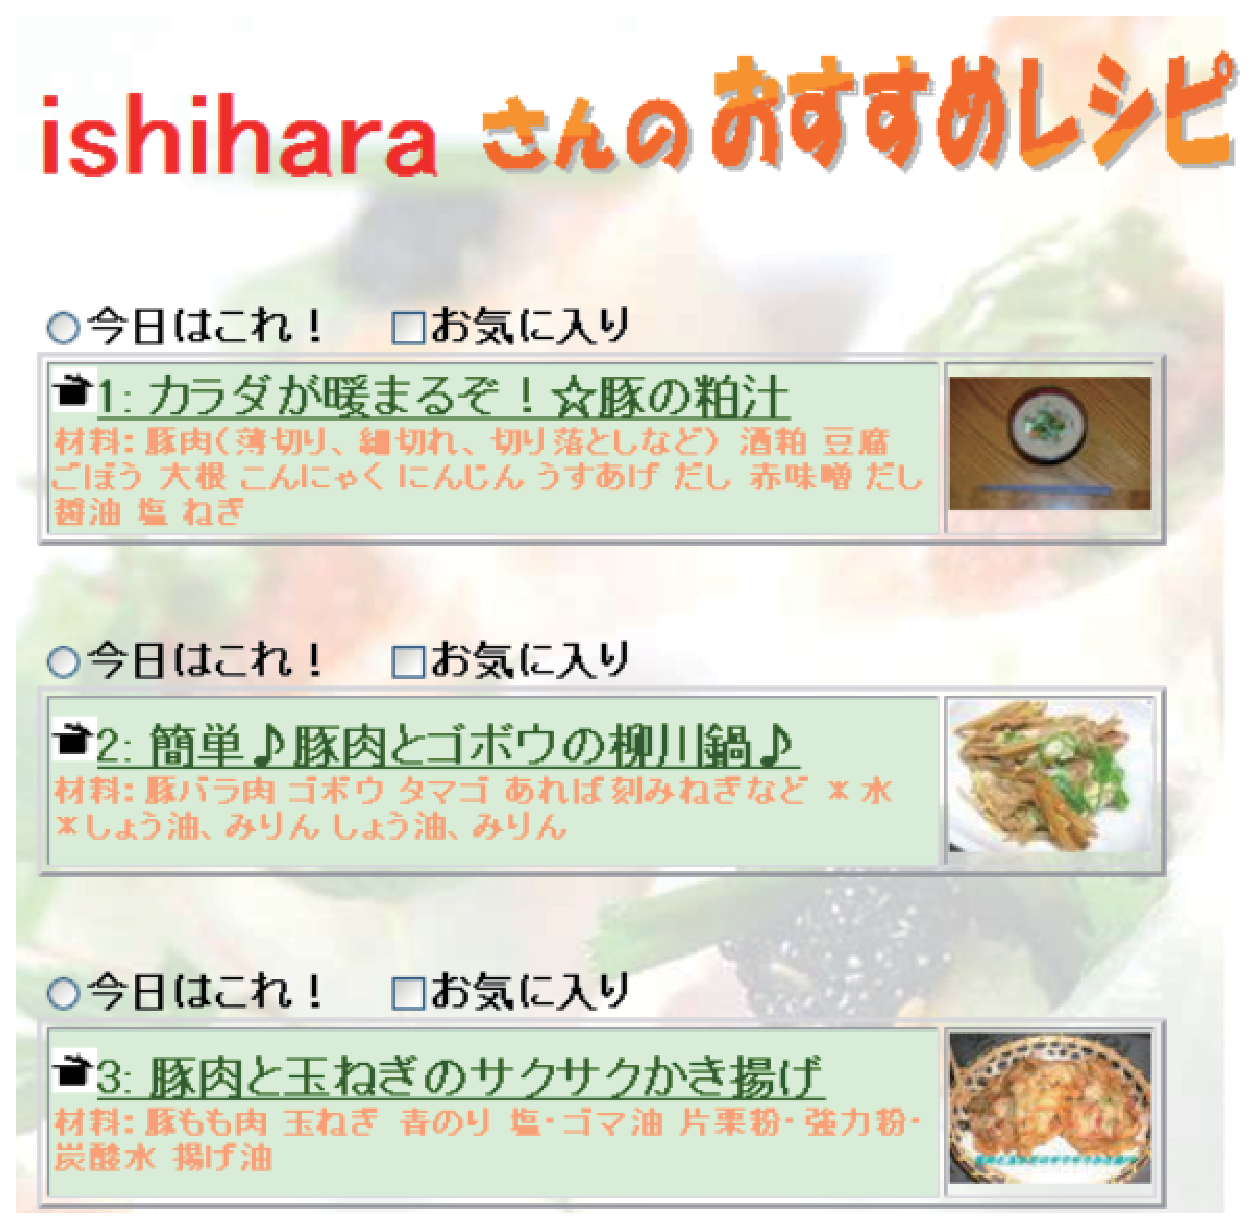
\includegraphics[clip,width=13cm]{resipi.eps}
    \caption[食材の利用履歴を利用したレシピ推薦システム]{食材の利用履歴を利用したレシピ推薦システム\cite{8}}
  \end{center}
\end{figure}

料理を推薦する際,どのような味が好きかという嗜好はとても重要な要素と考えられる.しかし,各店舗によって料理の味付け方法は異なり,
無数に存在する料理を実際に全部食べるということは不可能に近いため,味付けの分類が難しいという問題がある.

%--------------------------------------------------------------------

\chapter{推薦手法}
本章では,嗜好を用いて情報を推薦する手法について述べた後,本研究で用いる手法について述べる.

\section{嗜好を用いた情報推薦手法}
情報推薦に用いられる代表的な手法に,協調ベース型推薦,内容ベース型推薦,知識ベース型推薦がある\cite{9}.
それぞれの手法について以下で述べる.

\subsection{協調ベース型推薦}
協調ベース型推薦とは,類似したユーザの嗜好や過去の行動からユーザが好むであろうアイテムを推薦する手法である.
この手法は\cite{10}のおすすめなどショッピングサイトの商品推薦で用いられている.

以下に,協調ベース型推薦を用いて商品を推薦する例を示す.
表2.1は各ユーザの商品への嗜好を示している.この例ではユーザDに商品Dを推薦するのが適切かを判断する.
各ユーザの嗜好を比較すると,ユーザAとユーザDの嗜好が類似していることがわかる.
このことから,ユーザAが好きである商品DはユーザDも好むと予測できるため,ユーザDに商品Dを推薦することが適切だと判断するものである.

\begin{table}[htb]
  \begin{center}
  \scriptsize
    \caption{協調ベース型推薦を用いた商品を推薦する例}
    \normalsize
   \begin{tabular}{p{2.5cm}||p{2.5cm}|p{2.5cm}|p{2.5cm}|p{2.5cm}}
    \hline
ユーザ & 商品A & 商品B & 商品C & 商品D \\ \hline\hline
      ユーザA & 好き & 好き & 嫌い & 好き \\ \hline
      ユーザB & 好き & 嫌い & 好き & 好き \\ \hline
      ユーザC & 嫌い & 好き & 嫌い & 好き \\ \hline
      ユーザD & 好き & 好き & 嫌い & ? \\ \hline
  \end{tabular}
  \end{center}
\end{table}

\subsection{内容ベース型推薦}
内容ベース型推薦とは,ユーザの好むアイテムと類似したアイテムを推薦する手法である.

以下に,内容ベース型推薦を用いて料理を推薦する例を示す.
表2.2はユーザの好む料理の特徴と,各料理の特徴を示している.
この例ではユーザに新たな料理を推薦する際,どの料理を推薦するのが適切かを判断する.
ユーザと各料理の特徴を比較すると,料理Bの特徴とユーザの好む特徴が類似していることがわかる.
このことから,ユーザは料理Bも好むと予測できるため,料理Bを推薦することが適切だと判断するものである.

\begin{table}[htb]
  \begin{center}
  \scriptsize
    \caption{内容ベース型推薦を用いた料理を推薦する例}
    \normalsize
   \begin{tabular}{p{2.5cm}|p{2.5cm}||p{2.5cm}|p{2.5cm}|p{2.5cm}}
    \hline
    & ユーザ & 料理A & 料理B & 料理C  \\ \hline\hline
      ジャンル & 洋食 & 和食 & 洋食 & 和食 \\ \hline
      価格 & 1000円 & 800円 & 2000円 & 1000円 \\ \hline
      味 & 甘い & 辛い & 甘い & しょっぱい \\ \hline
  \end{tabular}
  \end{center}
\end{table}

\subsection{知識ベース型推薦}
知識ベース型推薦とは,ユーザに「予算は2000円,料理のジャンルは洋食が良い」など具体的な好みを示してもらい,示された好みを満たす商品に絞り込み,
ユーザへの効用が高くなるようにソートを行い,上位の商品を提示する手法である.
ユーザにあったソートを行うため,一般的な推薦システムで行われている人気順などのソートと比べ,推薦された商品に対するユーザの満足度が高くなるという特徴がある.

以下に,知識ベース型推薦を用いてカメラを推薦する例を示す.
表2.3は各カメラの特徴を示している.
この例ではユーザがカメラを選ぶ際に具体的な好みがある場合,どのカメラを推薦するのが適切かを判断する.
ユーザから「予算は30000円,5倍以上のズームができる,機能重視」という好みがあった場合,この条件を満たすカメラBとカメラDを推薦候補とする.
その後,推薦候補の中で「機能重視」という情報からソートを行い,カメラBを推薦リストの上位にすることが適切だと判断するものである.

\begin{table}[htb]
  \begin{center}
  \scriptsize
    \caption{知識ベース型推薦を用いたカメラを推薦する例}
    \normalsize
   \begin{tabular}{p{3.3cm}||p{3.3cm}|p{3.3cm}|p{3.3cm}}
    \hline
カメラ & 価格 & ズーム & 液晶サイズ \\ \hline\hline
      カメラA & 40000円 & 10倍 & 3インチ \\ \hline
      カメラB & 30000円 & 10倍 & 3インチ \\ \hline
      カメラC & 15000円 & 4倍 & 2.5インチ \\ \hline
      カメラD & 20000円 & 5倍 & 2.7インチ \\ \hline
  \end{tabular}
  \end{center}
\end{table}

\section{本研究で用いる手法}
本研究では,知識ベース型推薦を用いる.
その理由として,協調ベース型推薦を対象とする問題に用いた場合,料理の「価格」や「カテゴリ」などの属性を考慮した推薦を行えないという問題がある.
また,内容ベース型推薦を用いた場合,「地域らしい料理を食べる」という観光の際にのみ行われる稀な事象は嗜好情報を得ることが難しいという問題がある.
ユーザは料理や店舗の属性を考慮して料理を選択するため,ユーザの選択した属性と置かれた状況を考慮した推薦を行える知識ベース型推薦を用いて推薦を行う.

%--------------------------------------------------------------------
\chapter{提案手法}
本章では,本研究で用いたデータの収集について述べた後に,推薦アルゴリズムについて述べる.
最後に構築した知識ベース型推薦を用いた函館市の地域らしい料理を推薦するシステムの実装について述べる.


\section{使用するデータの収集}
本研究では,「食べログ」,「ぐるなび」からWebスクレイピングにより函館市の料理および飲食店の情報を収集した.
収集した情報の一部を表4.1,4.2,4.3に示す.
収集した情報は,飲食店の情報が2,206件,料理の情報が9,866件,口コミの情報が14,974件である.
他の属性として,料理に使われている材料の情報などを利用することを考えていたが,収集することが難しく,本研究では収集することができなかった.

\begin{table}[htb]
  \begin{center}
  \scriptsize
    \caption{収集した料理の情報}
    \normalsize
    \begin{tabular}{p{6cm}|p{6cm}}
    \hline
属性 & 値 \\ \hline\hline
      料理id & 5004 \\ \hline
      料理名 & 塩ラーメン \\ \hline
      価格(円) & 580 \\ \hline  \end{tabular}
  \end{center}
  \end{table}
  
\begin{table}[htb]
  \begin{center}
  \scriptsize
    \caption{収集した店舗の情報}
    \normalsize
   \begin{tabular}{p{6cm}|p{6cm}}
    \hline
属性 & 値 \\ \hline\hline
      店舗id & 347 \\ \hline
      店名 & 星龍軒 \\ \hline
      住所 &  北海道函館市若松町7-3\\ \hline
      オープン年(年)& 1951 \\ \hline
      ジャンル & ラーメン、餃子、中華料理 \\ \hline
      緯度 & 41.771268 \\ \hline
      経度 & 140.7264993 \\ \hline
  \end{tabular}
  \end{center}
\end{table}

\begin{table}[htb]
  \begin{center}
  \scriptsize
    \caption{収集した口コミの情報}
    \normalsize
   \begin{tabular}{p{6cm}|p{6cm}}
    \hline
属性 & 値 \\ \hline\hline
      口コミid &1284\\ \hline
      口コミ & 北海道にたくさん存在するご当地... \\ \hline
  \end{tabular}
  \end{center}
\end{table}


\section{推薦アルゴリズム}
本研究で用いた知識ベース型推薦のアルゴリズムを図4.1に示す.以下で詳細について述べる.

\begin{figure}[tbp]
  \begin{center}
    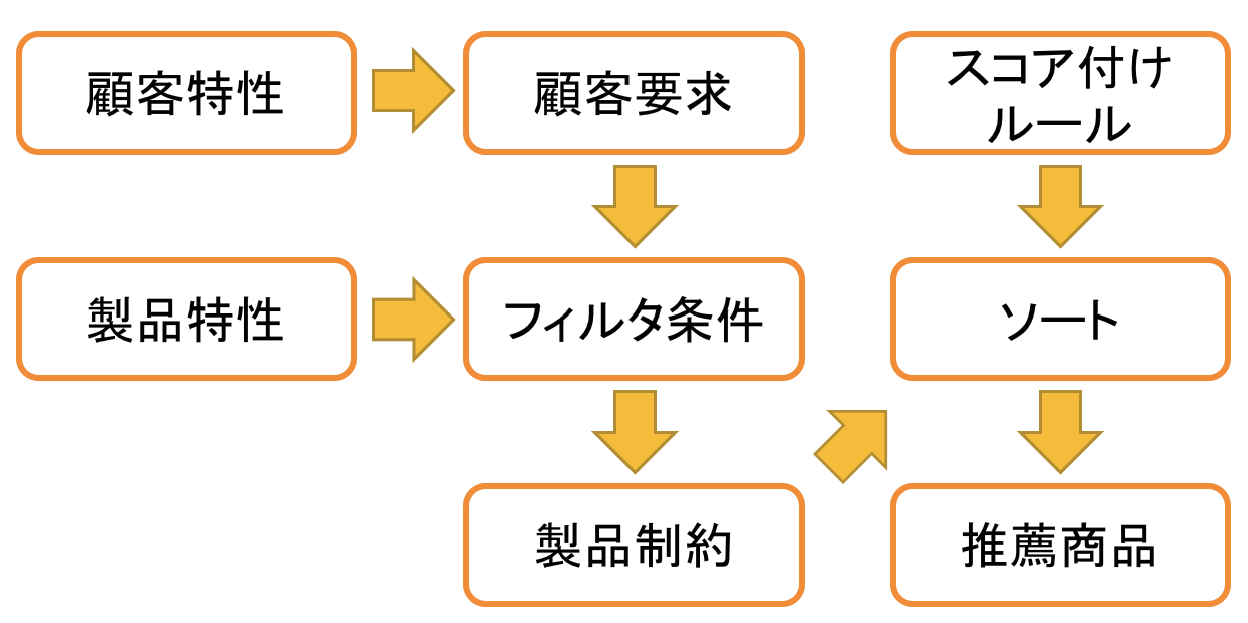
\includegraphics[clip,width=13cm]{model.eps}
    \caption{知識ベース型推薦のアルゴリズム}
  \end{center}
\end{figure}

\subsection{顧客要求}
知識ベース型推薦では,顧客特性をもとに顧客要求を設定する.
顧客特性とは,ユーザが商品を選ぶ際に使用する項目の集合である.本研究では顧客特性に,予算,ジャンルを使用する.
顧客要求とは,ユーザがどのような顧客特性を持っているかをまとめた集合である.本研究での顧客要求の例として「予算は1000円,ジャンルは洋食の料理が食べたい」が挙げられる.

\subsection{製品制約}
知識ベース型推薦では,顧客要求と製品特性をもとにフィルタ条件を用いて,ユーザが満たして欲しい条件を設定し,製品制約をする.
本研究において製品特性とは,料理及び店舗が持つすべての属性である.本研究で定義した製品特性は表4.1,4.2,4.3の属性である.
フィルタ条件とは,顧客要求と製品特性との関係を定義したものである.例えば,顧客要求として「予算が1000円」と入力された場合,「価格」が1000円以下の料理に絞り込む.
以上をもとに製品制約に使用するSQLを生成した.

\subsection{効用にもとづくソート}
知識ベース型推薦では,効用に基づくソートを行う.
本研究では,「地域発祥の料理」,「古くからある店舗」,「地域でしか食べられない料理」,「人気のある料理」の4項目の観点でユーザの効用を求め,ソートを行う.
金澤\cite{11}は観光における地域らしさには,地域の歴史・文化, 風土的特徴が関わっているとしている.このことから,料理における地域らしさを判断するには「地域発祥の料理」,「古くからある店舗」が必要と考えられるため観点とした.
また,「地域でしか食べられない料理」については,観光客は特定の地域でのみ食べられる料理かどうかで地域らしい料理と判断すると考えられるため観点とした.
「人気のある料理」については人気のある料理かどうかで地域らしい料理と判断すると考えられるため観点とした.

効用は式4.1で求めることができる.

\begin{equation}
効用(p)=\sum_{j=1}^{n} 関心度(j)×貢献度(p,j) 
\end{equation}

{\it p}は料理,{\it j}は観点を表す.関心度とはある観点においてどれほど製品に関心があるのかを表した度合いである.
本研究では関心度をユーザに設定してもらう.関心度の値は0から1の範囲とした.貢献度とは製品がある観点にどれだけ貢献しているかを表した度合いである.
本研究ではスコア付けルールを用いて貢献度を設定する.スコア付けルールとは料理および店舗の属性をもとに本研究で定義した観点を数値化するものである.貢献度の値は0から10の範囲とした.
以下に,各観点の貢献度の求め方を示す.

\subsubsection{地域発祥の料理}
地域発祥の料理の貢献度は,製品特性の料理名とJAPAN WEB MAGAZINE\cite{12},Wikipedia\cite{13}を用いて定義した.
料理の発祥した地域が函館に近いほど貢献度を高くする.表4.4に発祥地域と貢献度の値の関係を示す.

\begin{table}[htb]
  \begin{center}
  \scriptsize
    \caption{発祥地域と貢献度の値の関係}
    \normalsize
   \begin{tabular}{p{6cm}|p{6cm}}
    \hline
発祥地域 & 貢献度の値 \\ \hline\hline
      函館市 & 10  \\ \hline
      渡島管内 & 7 \\ \hline
      道南地域 & 5 \\ \hline
      北海道 & 3 \\ \hline
      その他 & 0 \\ \hline
  \end{tabular}
  \end{center}
\end{table}

\subsubsection{古くからある店舗}
古くからある店舗の貢献度は,製品特性のオープン年を用いて定義した.
店の開店した年が昔であるほど貢献度を高くする.表4.5に開店した年と貢献度の値の関係を示す.

\begin{table}[htb]
  \begin{center}
  \scriptsize
    \caption{開店した年と貢献度の値の関係}
    \normalsize
   \begin{tabular}{p{6cm}|p{6cm}}
    \hline
開店した年(年) & 貢献度の値 \\ \hline\hline
      〜1900 & 10  \\ \hline
      1901〜1950 & 7 \\ \hline
      1951〜2000 & 4 \\ \hline
      2001〜 & 0 \\ \hline
  \end{tabular}
  \end{center}
\end{table}

\subsubsection{地域でしか食べられない料理}
地域でしか食べられない料理の貢献度は,製品特性の料理名と2.1節で説明した手法を用いて定義した.
地域のメニューと首都圏のメニューを比較し,首都圏で地域のメニューを取り扱っている店舗数が少ないほど貢献度を高くする.
表4.6に取り扱っている店舗数と貢献度の値の関係を示す.

\begin{table}[htb]
  \begin{center}
  \scriptsize
    \caption{取り扱っている店舗数と貢献度の値の関係}
    \normalsize
   \begin{tabular}{p{6cm}|p{6cm}}
    \hline
取り扱っている店舗数(店舗) & 貢献度の値 \\ \hline\hline
      〜3 & 10  \\ \hline
      4〜6 & 8 \\ \hline
      7〜9 & 6 \\ \hline
      10〜12 & 4 \\ \hline
      13〜15 & 2 \\ \hline
     16〜 & 0 \\ \hline
  \end{tabular}
  \end{center}
\end{table}

\subsubsection{人気のある料理}
人気のある料理の貢献度は,製品特性の口コミを用いて定義した.
まず,人気のあるお店かどうかを判断するため,口コミの数で0から5の範囲の貢献度を決める.口コミの数が多いほど貢献度を高くする.表4.7に口コミの数と貢献度の値の関係を示す.
続いて,人気の料理かどうかを判断するため,口コミに登場する割合で0から5の範囲の貢献度を決める.口コミに登場する割合が高いほど貢献度を高くする.表4.8に口コミに登場する割合と貢献度の値の関係を示す.
この2つの値を足した数値を人気のある料理の貢献度とする.

\begin{table}[htb]
  \begin{center}
  \scriptsize
    \caption{口コミの数と貢献度の値の関係}
    \normalsize
   \begin{tabular}{p{6cm}|p{6cm}}
    \hline
口コミの数(件) & 貢献度の値 \\ \hline\hline
      250〜 & 5  \\ \hline
      200〜249 & 4 \\ \hline
      150〜199 & 3 \\ \hline
      100〜149 & 2 \\ \hline
      50〜99 & 1 \\ \hline
     〜49 & 0 \\ \hline
  \end{tabular}
  \end{center}
\end{table}

\begin{table}[htb]
  \begin{center}
  \scriptsize
    \caption{口コミに登場する割合と貢献度の値の関係}
    \normalsize
   \begin{tabular}{p{6cm}|p{6cm}}
    \hline
口コミに登場する割合(\%) & 貢献度の値 \\ \hline\hline
      80〜100 & 5  \\ \hline
      60〜79 & 4 \\ \hline
      40〜59 & 3 \\ \hline
      20〜39 & 2 \\ \hline
      10〜19 & 1 \\ \hline
      0〜10 & 0 \\ \hline
  \end{tabular}
  \end{center}
\end{table}

\section{システムの実装}
本研究では4.1,4.2節をもとにWeb上で利用できるフードツーリズム支援システムを構築した.提案システム画面を図2に示す.
ユーザの要求を入力する手段として,セレクトボックス,テキストボックス,スライダを用いる.
セレクトボックスはカテゴリを入力するため,テキストボックスは予算を入力するため,スライダーは各観点への関心度を入力するために用いた.
料理を推薦する箇所は,ページにアクセスした際にはランダムで8件推薦され,要求を入力し終えたタイミングで自動的にユーザへの効用が高い上位8件を推薦する.
加えて,推薦された料理を取り扱っている店舗の場所がわかるように,マップにマーカーを設置し店舗の位置を表示する.

\begin{figure}[tbp]
  \begin{center}
    \includegraphics[clip,width=13cm]{start.eps}
    \caption{システム画面(初期)}
  \end{center}
\end{figure}

\newpage

\begin{figure}[tbp]
  \begin{center}
    \includegraphics[clip,width=13cm]{after.eps}
    \caption{システム画面(入力後)}
  \end{center}
\end{figure}

%--------------------------------------------------------------------
\chapter{実験}
本章で提案システムの有用性を確認するために行った実験の概要と方法,結果を述べた後に,
結果から得られた考察を述べる.

\section{実験概要}
本研究の目的は,観光客の嗜好と置かれた状況を考慮した地域らしい料理の推薦を行うことで観光客の満足度向上を目指すことである.
そのため,グルメサイトと比較した際に地域らしい料理を探しやすいかどうか,および提案システムの評価をするために実験を行った.
被験者は本学の学生9人とした.

\section{実験方法}
\subsection{グルメサイトとの比較実験}
本実験の目的は提案システムをグルメサイトと比較した際に,地域らしい料理が探しやすいか調査することを目的としている.
まず,被験者に「食べログ」と「ぐるなび」,提案システムを用いて観光に来た際に食べてみたい料理を選んでもらう.
被験者の状況は函館に来る予定の観光者で,何か地域らしい料理を探していることとした.
「食べログ」を用いて料理を選ぶ方法を手法1,「ぐるなび」を用いて料理を選ぶ方法を手法2,提案システムを用いて料理を選ぶ方法を手法3とする,
全ての手法で食べてみたい料理を選んでもらった後,以下のアンケートに回答してもらった.

\begin{itemize}
 \item どの方法で探すのが一番簡単でしたか?(3択)
 \item どの方法で選んだ料理が一番魅力的でしたか?(3択)
\end{itemize}

\subsection{提案システムの実験}
本実験の目的は提案システムにて推薦される料理がユーザの入力した項目にあっているか,地域らしい料理に求める観点は過不足ないかの2つを調査することを目的としている.
本実験では,被験者に提案システムを自由に使ってもらった後,以下のアンケートに回答してもらった.

\begin{itemize}
 \item 入力した項目にあった料理が推薦されていますか?(4段階)
 \item 以下の項目で地域らしい料理を探したことがありますか?(「はい」か「いいえ」)
 \begin{itemize}
 \item 地域発祥の料理
  \item 古くからある店舗
   \item 地域でしか食べられない料理
    \item 人気のある料理
  \end{itemize}
 \item 地域らしい料理を探す際に重視している項目は他に何かありますか?(自由記述)
 \end{itemize}

\section{結果}
\subsection{グルメサイトとの比較実験}
「どの方法で探すのが一番簡単でしたか?」のアンケート結果を図5.1,「どの方法で選んだ料理が一番魅力的でしたか?」を図5.2に示す.
「どの方法で探すのが一番簡単でしたか?」において,「手法1」と答えた人は2人,「手法2」と答えた人は0人,「手法3」と答えた人は7人であった.
「どの方法で選んだ料理が一番魅力的でしたか?」において,「手法1」と答えた人は5人,「手法2」と答えた人は0人,「手法3」と答えた人は4人であった.

\begin{figure}[tbp]
  \begin{center}
    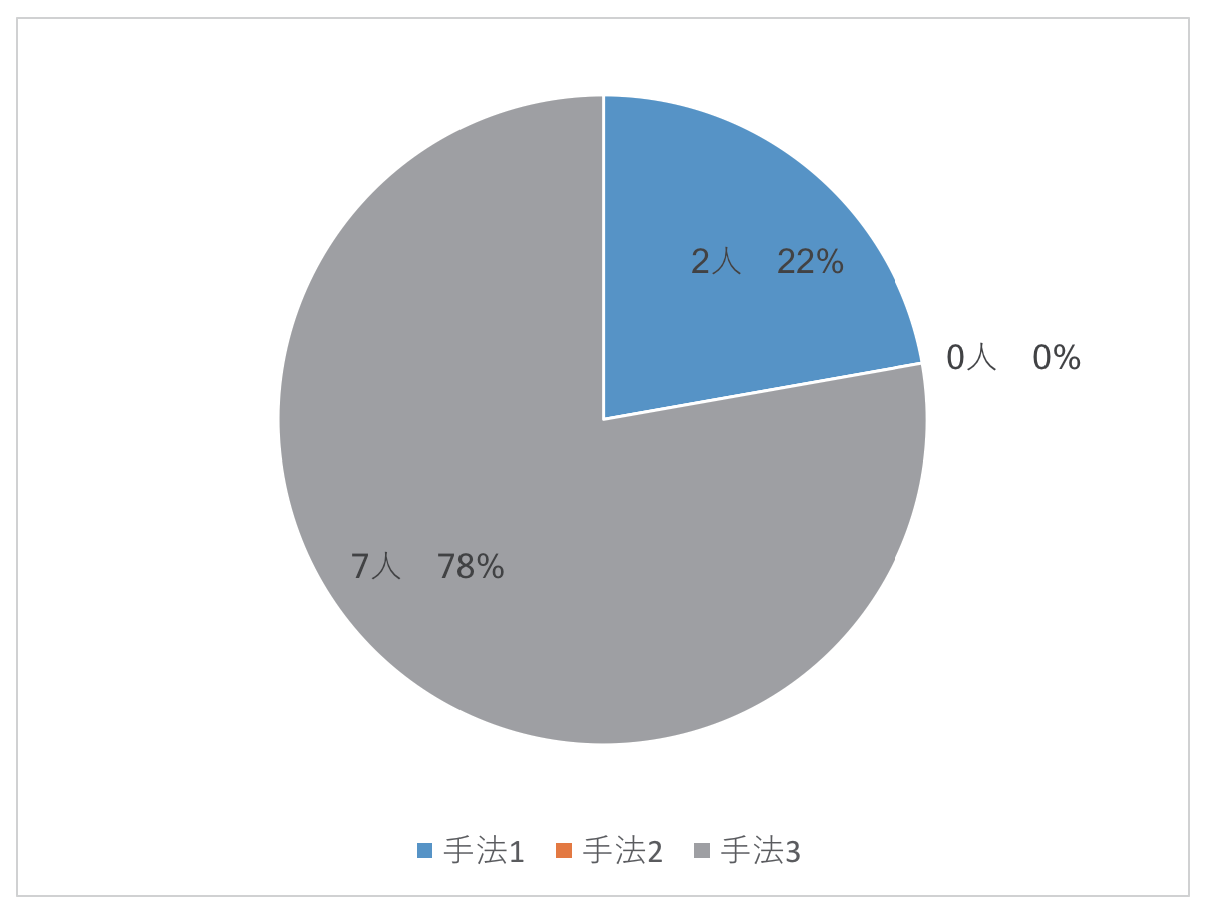
\includegraphics[clip,width=12cm]{5.1.eps}
    \caption[「どの方法で探すのが一番簡単でしたか?」のアンケート結果]{「どの方法で探すのが一番簡単でしたか?」のアンケート結果(N=9)}
  \end{center}
\end{figure}

\begin{figure}[tbp]
  \begin{center}
    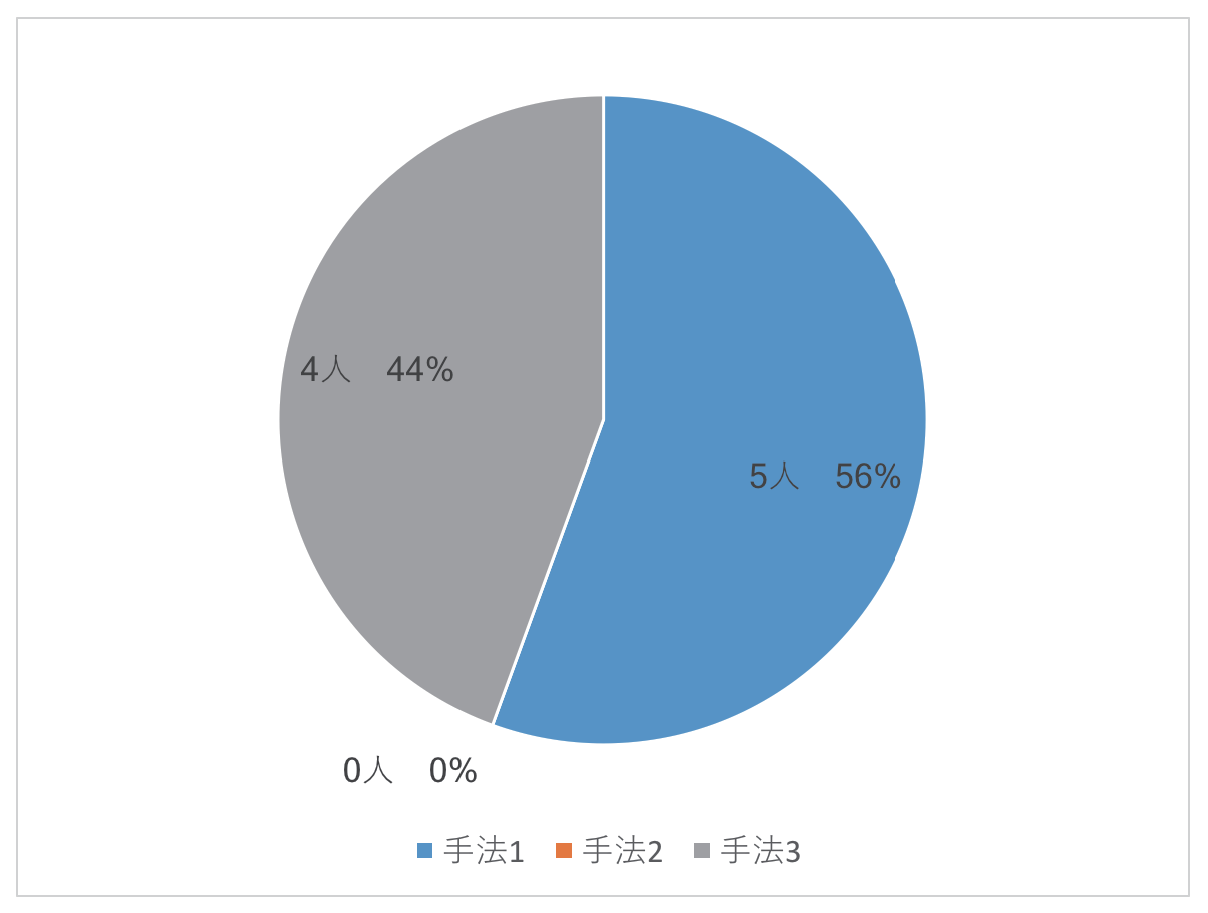
\includegraphics[clip,width=12cm]{5.2.eps}
    \caption[「どの方法で選んだ料理が一番魅力的でしたか?」のアンケート結果]{「どの方法で選んだ料理が一番魅力的でしたか?」のアンケート結果(N=9)}
  \end{center}
\end{figure}


\subsection{提案システムの実験}
「入力した項目にあった料理が推薦されていますか?」のアンケート結果を図5.3,
「以下の項目で地域らしい料理を探したことがありますか?」を図5.4,5.5,5.6,5.7,「地域らしい料理を探す際に重視している項目は他に何かありますか?」を表5.1に示す.
「入力した項目にあった料理が推薦されていますか?」において, 「されている」,「だいたいされている」と答えた人は7人,「あまりされていない」,「されていない」と答えた人は2人であった.
「以下の項目で地域らしい料理を探したことがありますか?」において,
「地域発祥の料理」に「はい」と答えた人は8人,「いいえ」と答えた人は1人,
「古くからある店舗」に「はい」と答えた人は 0人,「いいえ」と答えた人は9人,
「 地域でしか食べられない料理」に「はい」と答えた人は6人,「いいえ」と答えた人は3人,
「人気のある料理」に「はい」と答えた人は9人,「いいえ」と答えた人は0人であった.
「地域らしい料理を探す際に重視している項目は他に何かありますか?」において,1件の回答が得られた.

\begin{figure}[tbp]
  \begin{center}
    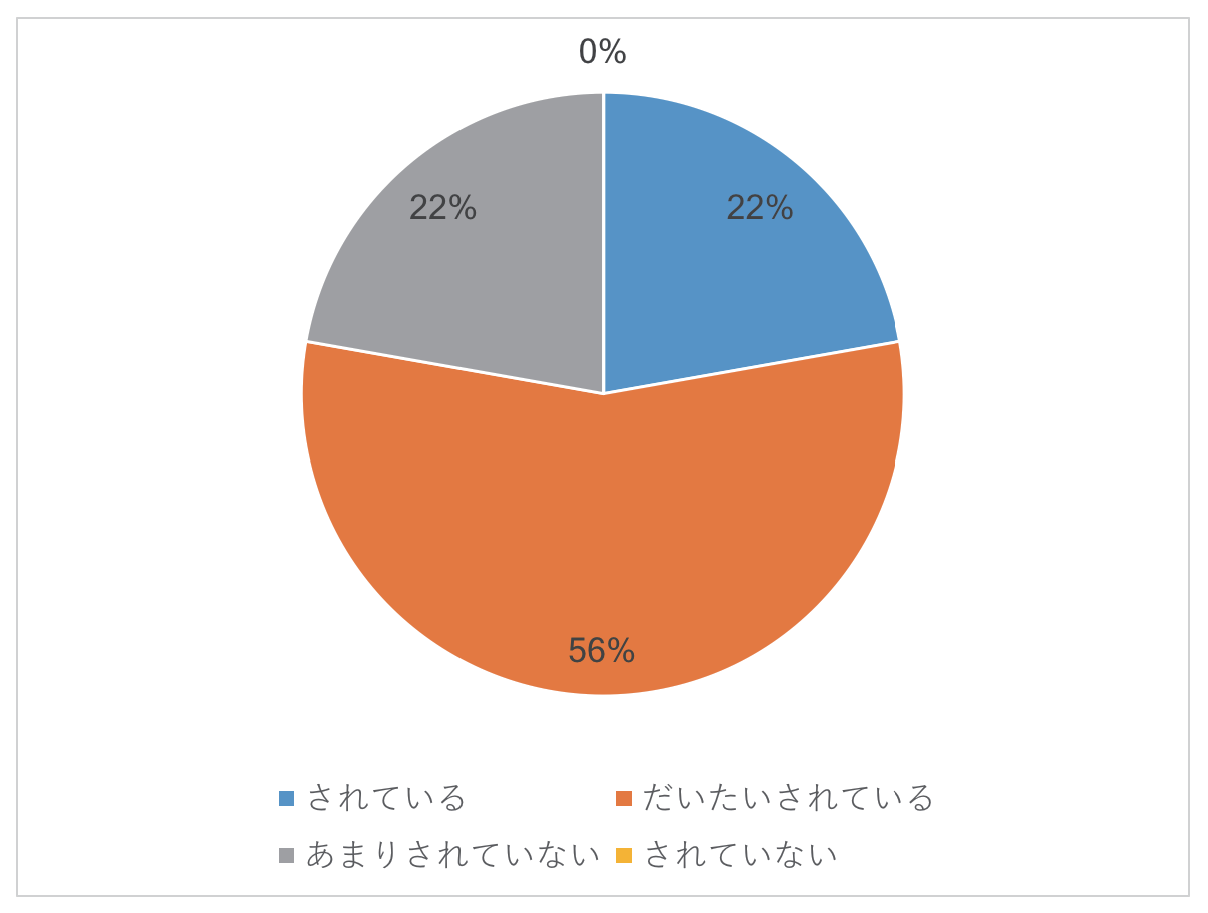
\includegraphics[clip,width=12cm]{5.3.eps}
    \caption[「入力した項目にあった料理が推薦されていますか?」のアンケート結果]{「入力した項目にあった料理が推薦されていますか?」のアンケート結果(N=9)}
  \end{center}
\end{figure}

\begin{figure}[tbp]
  \begin{center}
    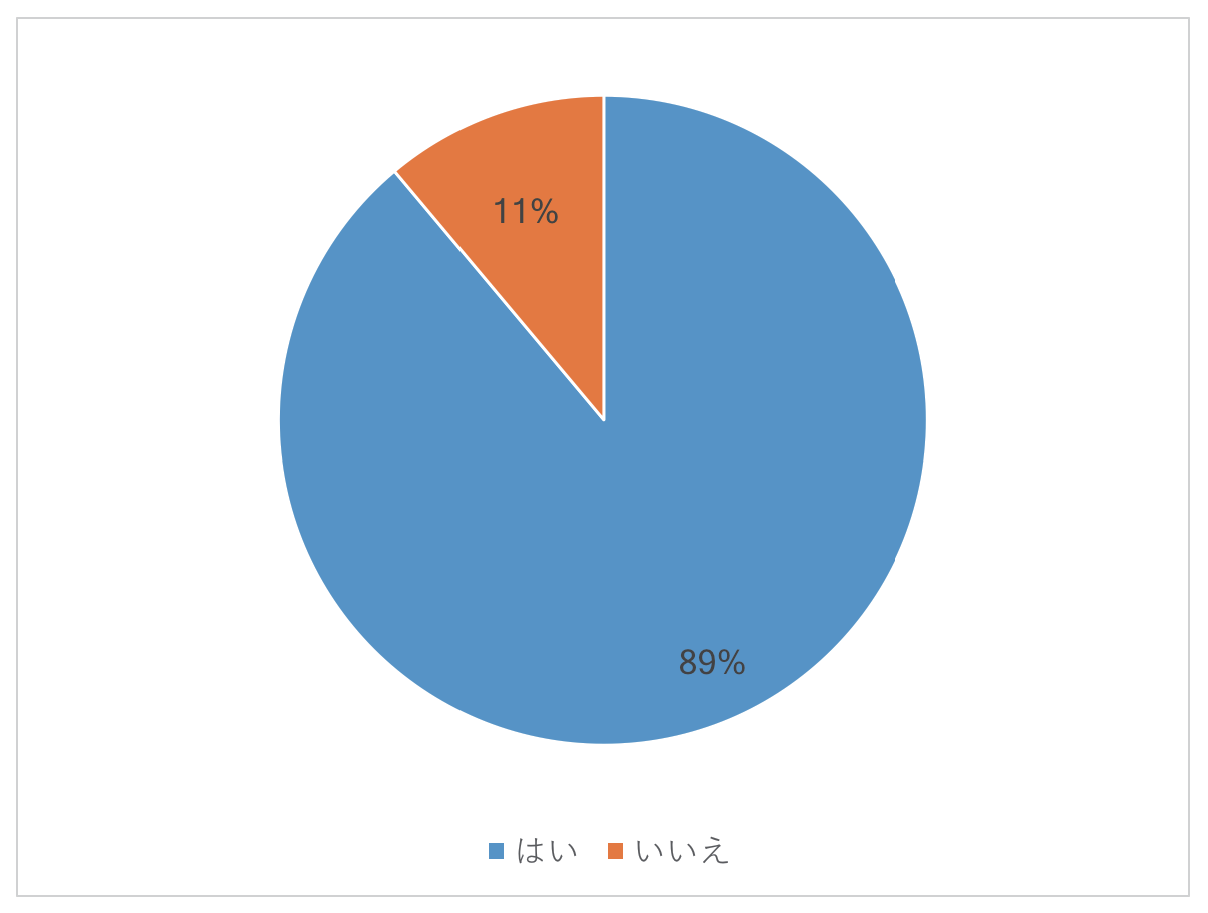
\includegraphics[clip,width=12cm]{5.4.eps}
    \caption[「地域発祥の料理」のアンケート結果]{「地域発祥の料理」のアンケート結果(N=9)}
  \end{center}
\end{figure}

\begin{figure}[tbp]
  \begin{center}
    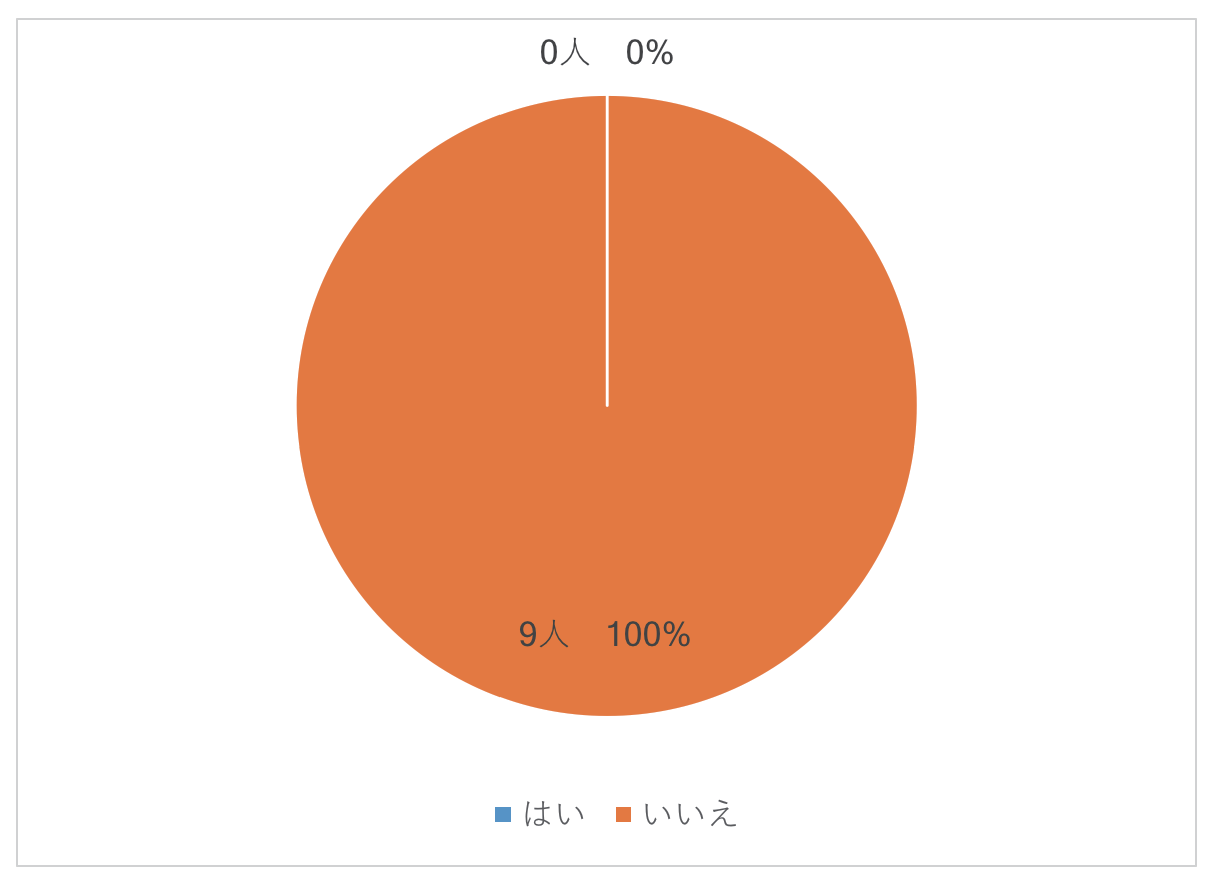
\includegraphics[clip,width=12cm]{5.5.eps}
    \caption[「古くからある店舗」のアンケート結果]{「古くからある店舗」のアンケート結果(N=9)}
  \end{center}
\end{figure}

\begin{figure}[tbp]
  \begin{center}
    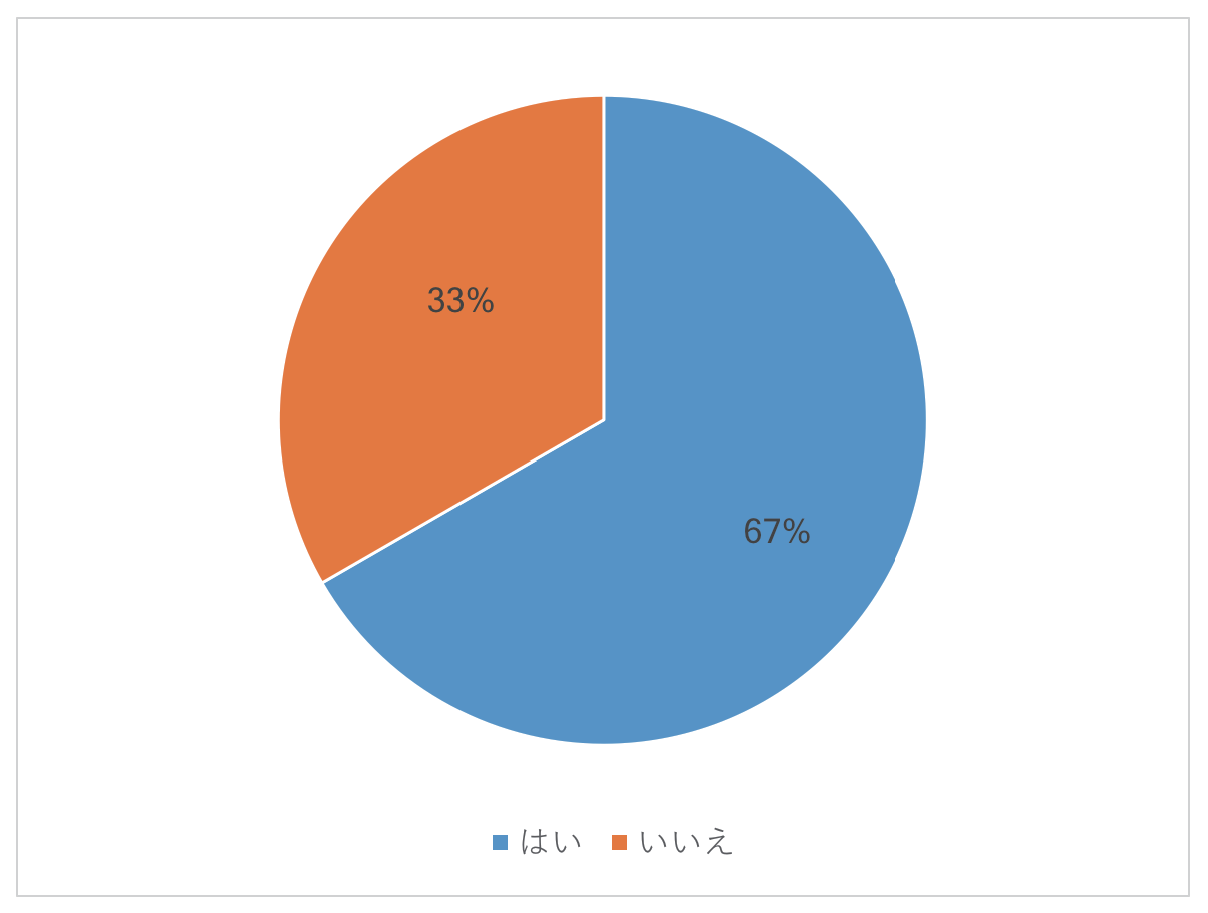
\includegraphics[clip,width=12cm]{5.6.eps}
    \caption[「 地域でしか食べられない料理」のアンケート結果]{「 地域でしか食べられない料理」のアンケート結果(N=9)}
  \end{center}
\end{figure}

\begin{figure}[tbp]
  \begin{center}
    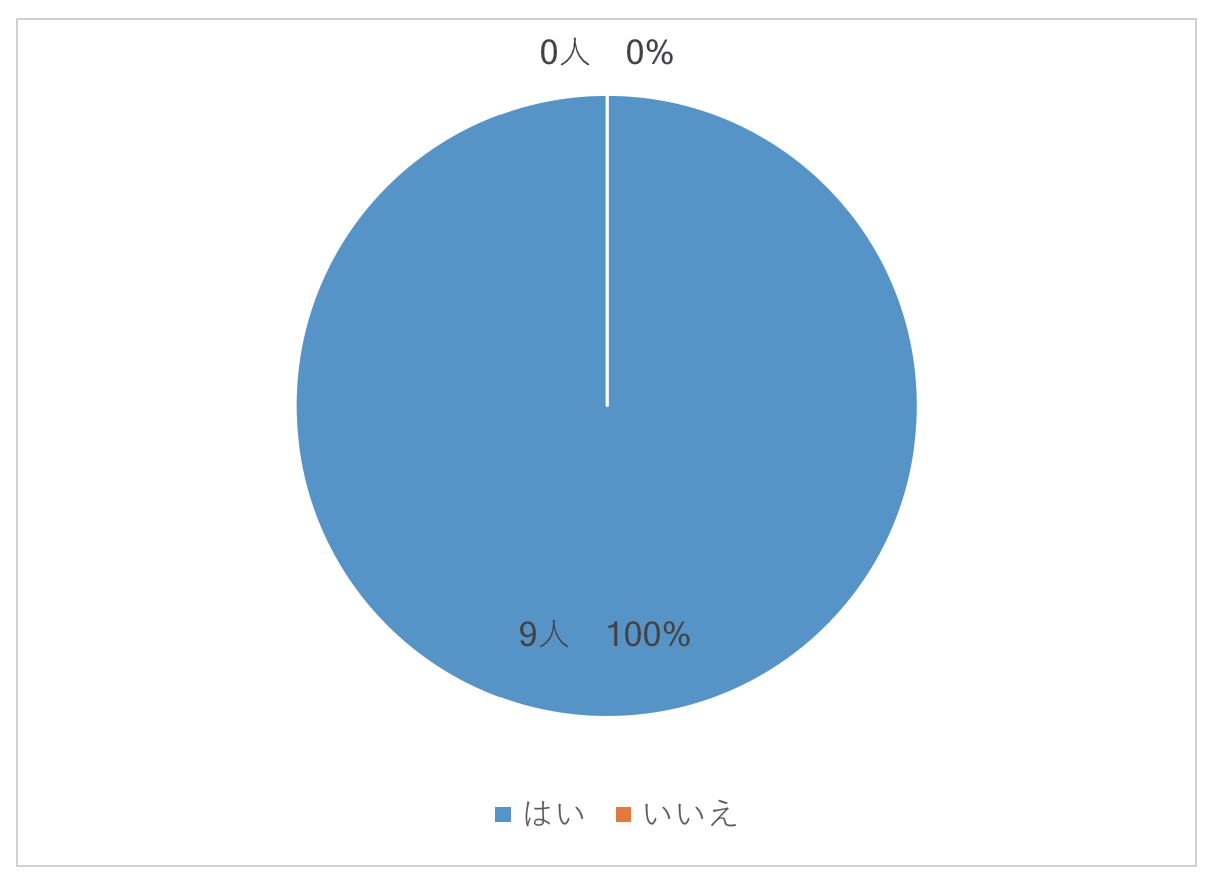
\includegraphics[clip,width=12cm]{5.7.eps}
    \caption[「人気のある料理」のアンケート結果]{「人気のある料理」のアンケート結果(N=9)}
  \end{center}
\end{figure}

\begin{table}[htb]
  \begin{center}
  \scriptsize
    \caption[「地域らしい料理を探す際に重視している項目は他に何かありますか?」のアンケート結果]{「地域らしい料理を探す際に重視している項目は他に何かありますか?」のアンケート結果(N=1)}
    \normalsize
   \begin{tabular}{p{13cm}}
    \hline
 具体的な食べ物名が決まっている時がある(函館ならイカ)\\ \hline
  \end{tabular}
  \end{center}
\end{table}

\section{考察}
\subsection{グルメサイトとの比較実験}
「どの方法で探すのが一番簡単でしたか?」について比較すると,手法3と答えた人数が手法1,2よりも多かった.
また,「どの方法で選んだ料理が一番魅力的でしたか?」について比較すると,手法1,2と答えた人数がほぼ同数であった.
このことから,提案システムは既存のグルメサイトよりも簡単に地域らしい料理を探せ,グルメサイトと同じほど魅力的なものを見つけることができると考えられる.

\subsection{提案システムの実験}
「入力した項目にあった料理が推薦されていますか?」では,75\%以上の人が良い評価をした.このことから,推薦される料理はユーザの入力した項目にほぼあっていると考えられる.
「以下の項目で地域らしい料理を探したことがありますか?」では,「古くからある店舗」以外の項目では「はい」と答えた人の割合が多かった.
このことから,「古くからある店舗」は地域らしい料理に求める観点にあまり必要ないことが考えられる.
「地域らしい料理を探す際に重視している項目は他に何かありますか?」では,具体的に食べたい料理名が決まっている場合には提案システムでは要求を入力する項目が不足していることがわかった.
このことから,料理名を用いた推薦をできるように項目を追加する必要があると考えられる.

%--------------------------------------------------------------------
\chapter{結論}
本章では,本研究のまとめと,今後の展望を述べる.

\section{まとめ}
本研究では,観光客が地域らしい料理を探すことは容易ではないという問題を解決するために,観光客の嗜好と置かれた状況を考慮した地域らしい料理の推薦を行うことで観光客の満足度向上を目指した.
そのために,本研究では知識ベース型推薦を用いた函館市の地域らしい料理を推薦するシステムを提案した.実験の結果,提案システムはグルメサイトと比べ地域らしい料理を探しやすいことがわかった.
しかし,本研究で定義した地域らしい料理に求める項目では過不足があり,ユーザの要望を十分に考慮出来ていないため,改善する必要があるとわかった,

\section{今後の展望}
実験結果からの考察をもとに,提案手法の改善を行う必要がある.具体的には,料理名を用いた推薦を行えるようにする必要がある.
提案システムでは,具体的に食べたい料理名が決まっている観光客である場合,要求を入力する箇所がなかった.また,観光客があまり気にしない項目を入力できるようにしていた.
これらの問題を解決するために,本研究で定義した地域らしい料理に求める項目の修正が必要だと考えられる.

\chapter *{謝辞}
本研究にあたりご指導いただいた指導教員の奥野拓准教授に深くお礼申し上げます.
また,様々な助言をしていただいた奥野研究室の皆様,本研究に関わった方々にも深くお礼申し上げます.



%--------------------------------------------------------------------
% 参考文献
\begin{thebibliography}{99}
\bibitem{1} 観光庁 : ニューツーリズムの振興(オンライン), \url{http://www.mlit.go.jp/kankocho/page05_000044.html}(2018/1/20 アクセス).
\bibitem{2} リクルートじゃらんリサーチセンター : じゃらん宿泊旅行調査(オンライン), \url{http://jrc.jalan.net/j/surveys.html}(2018/1/20 アクセス).
\bibitem{3} 日本フードツーリズム協会 : \url{http://food-tourism.jp}(2018/1/20 アクセス).
\bibitem{4} 食べログ : \url{https://tabelog.com}(2018/1/20 アクセス).
\bibitem{5} ぐるなび : \url{https://www.gnavi.co.jp}(2018/1/20 アクセス).
\bibitem{6} 宇部雅彦,村田嘉利,鈴木彰真 : 地域特産メニュー抽出手法の提案, 情報処理学会第76回全国大会 (2014).
\bibitem{7} 樽井勇介:協調フィルタリングとコンテンツ分析を利用した観光地推薦手法の検討,上武大学経営情報学部紀要,第 36 号,pp. 1-14(2011).
\bibitem{8} 上田真由美,石原和幸,平野靖,梶田将司,間瀬 健二:食材利用履歴に基づき個人の嗜好を反映 するレシピ推薦手法,日本データベース学会 Letters,Vol.6,No.4,pp. 29-32(2008).
\bibitem{9} D.Jannach,M.Zanker,A.Felferning,G.Friedrich:情報推薦システム入門-理論と実践-, pp. 82-124 (2012).
\bibitem{10} Amazon : \url{https://www.amazon.co.jp}(2018/1/20 アクセス).
\bibitem{11} 金澤成保:「京都らしさ」、「地域らしさ」を問う,JUDI関西(オンライン),\url{http:// judi.sub.jp/judi/f17/a07kana.pdf}(2018/1/20 アクセス).
\bibitem{12} JAPAN WEB MAGAZINE : \url{http://japan-web-magazine.com}(2018/1/20 アクセス).
\bibitem{13} Wikipedia : \url{http://wikipedia.org}(2018/1/20 アクセス).
\end{thebibliography}

% 表目次の表示
\listoftables

% 図目次の表示
\listoffigures

\end{document}
